\chapter{Proposed System for Sketch Understanding}
\section{Aims of the System}
\label{sec:AimsOfTheSystem}
The previous chapter shows the current trends in sketch recognition. This thesis introduce a solution for the problem that give optimize solution for the segmentation problem. Particle swarm optimization is used to correctly segment strokes into curves and lines. The current implemented system either segment strokes based on simple curvature data or using some more complex algorithm. The performance of most algorithms are based on user style. 

% Stroke segmentation is one of the most complex problems in the sketch recognition system. It is dividing the   
%In stroke segmentation problem is  Particle swarm optimization is used as the 

\section{An Overview of the System}
\label{sec:AnOverviewOfTheSystem}
   This research solve sketch segmentation optimization problem using particle swarm algorithm PSO.  Due to sloppiness of users and hardware glitches the system process the data before segmentation to generate a set of possible corner or critical points.  The clustering algorithm then tries to group the segments together to form a single symbol. A set of features is extracted from the symbols to be used by the classifier.  %The stroke is the path of points from the instant the pen is down till it is up.
The block digram in fig. \ref{fig:Blockdiagram} shows that the main system blocks are 1) preprocessing, 2) segmentation, 3) clustering, 4) feature extraction, and finally 5) classification. The next section will describe each component in details. 
 %Due to sloppiness of users and hardware glitches the system processes the data before further
\begin{figure}[]
	\centering
		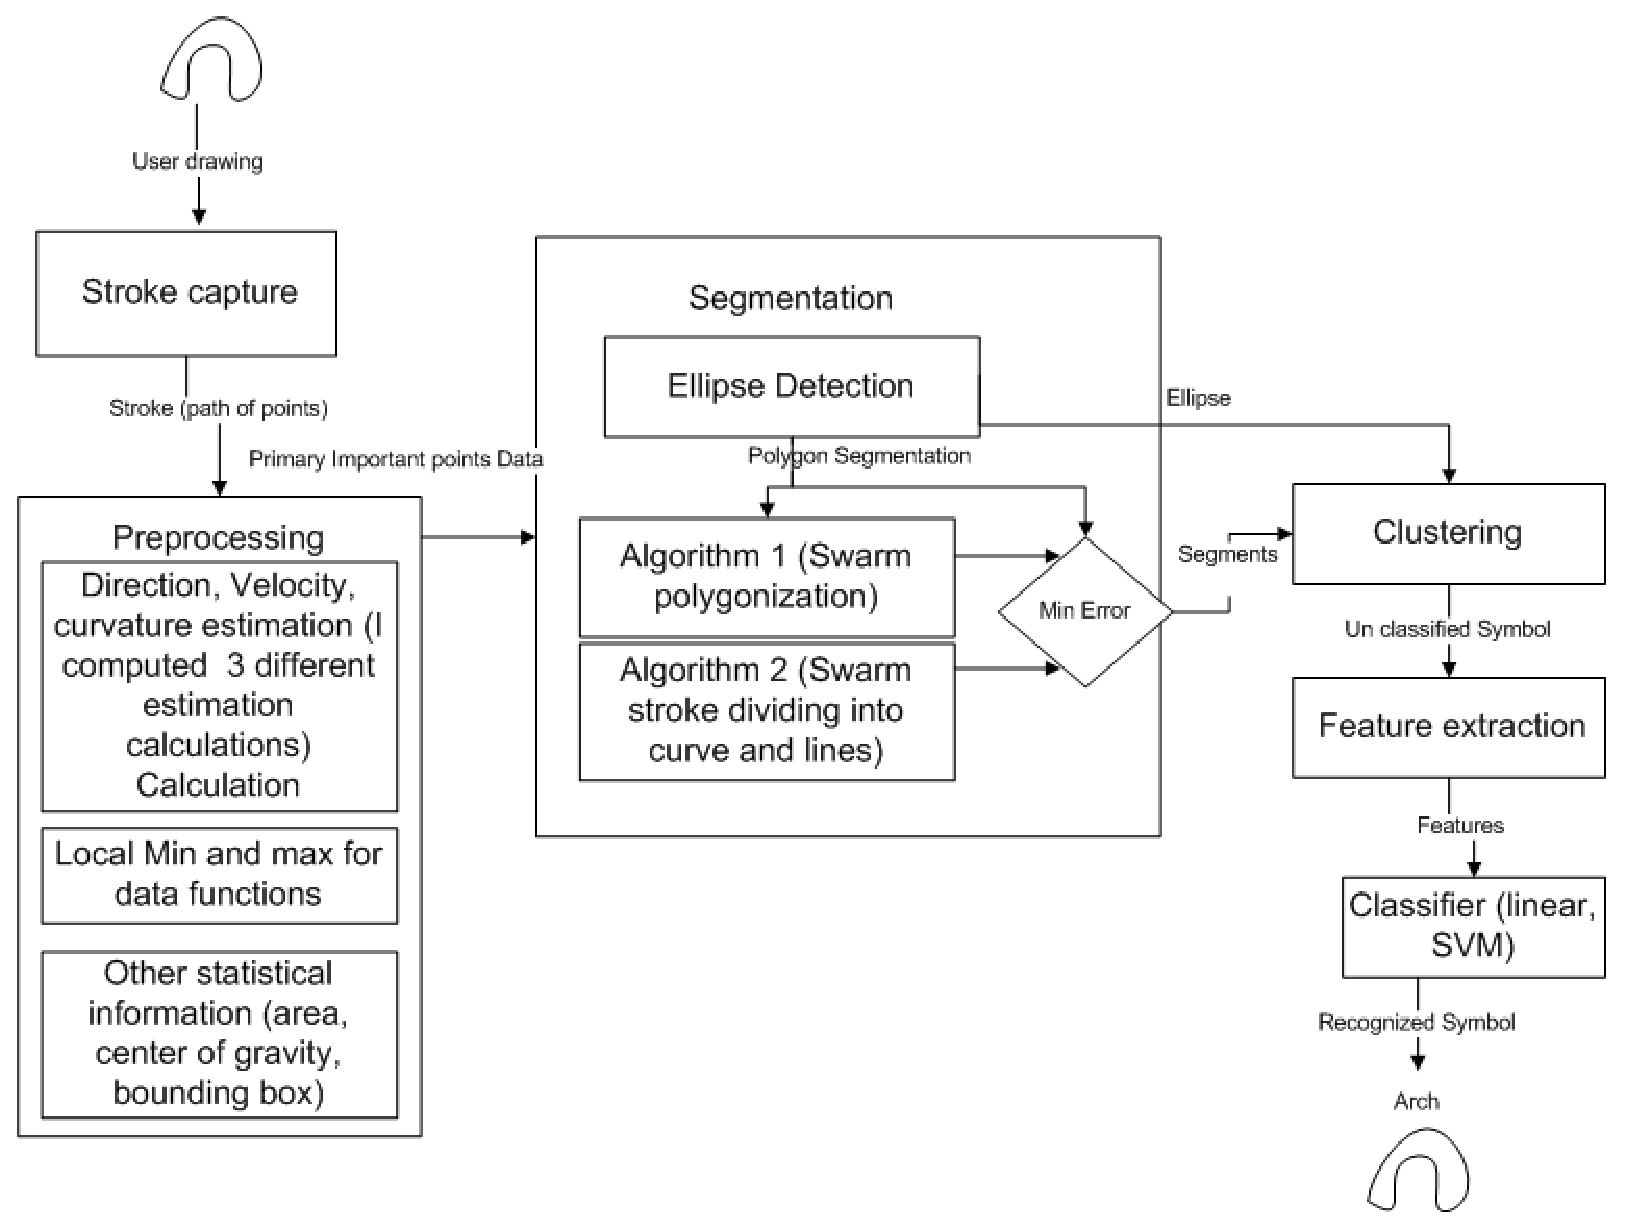
\includegraphics[scale=0.6]{images/Blockdiagram.eps}
	\caption[  ]{The system Block Diagram}
	\label{fig:Blockdiagram}
\end{figure}
 

\section{System Components}
\label{sec:SystemComponents}
 
The \textbf{preprocessing} is responsible of capturing the input data and removing the noise from it. The preprocessing block as in fig.  \ref{fig:Blockdiagram}   is consistent of  some calculation based on    the time differences, direction, speed and curvature of all points of the stroke. After computing these data is the local minimum and local maximum of each information is extracted from the data computed. The remaining of the geometrical and statistical data is then evaluated from the stroke.  The system then proceeds to estimate a set of possible dominant points to help in the segmentation process.   \\
 
  
The  next step is \textbf{segmentation}, the goal of the segmentation stage is to divide stroke into segments of either curves or lines. The segmentation process is divided into two steps ellipse fitting and curve segmentation. In the first step, the ellipse fitting process tries to fit the stroke into an ellipse. If the system fails it passes the stroke to the second step; curve segmentation which consist of two PSO segmentation algorithms. The two algorithms will generate two segmentations, the system will choose the segmentation that has the minimum segmentation error.%  generate the segmentations,  the minimum error will be the chosen segmentation. % is the ellipse fitting

 %the stroke first If the ellipse detection fails the stroke is passed to the segmentation algorithms which will pass it to the two PSO algorithms described below the segmentation with the minimum error will be the chosen segmentation.  The segmentation is then added to the set of un-recognized segments in the system. \\% This part is repeated for each stroke. 
 The clustering algorithms starts to group segments together after the segmentation step. The system let the user draws the symbol by using any number of strokes, a set of unrecognized segments is passed to the clustering algorithm to generate a symbol and compute a feature vector for it.
 
 Feature Extraction is the fourth block in the system. he system compute composite set of features some are statistical other are spatial features based on the type primitives.%The system extract segment based and statistical based features from the set of segments that the clustering algorithms produce. 
  
   The final step is a SVM classifier that will use the features computed to classify the segments into one of the previously trained classes. %  Or to determine the symbol of the given segments from the set of preciously trained symbols. 
 
 %with a symbol from the training set.% The system compute composite set of features some are statistical other are spatial features based on the type primitives. Finally, the strokes are classified into the corresponding classes.% the classifier identifies the strokes into a symbol from the set of known symbols.\\

\chapter{System Details}
\label{sec:SystemDetails}


\section{Preprocessing}
\label{sec:Preprocessing}
%Some data is extracted from the points in the stroke.
 It is noted that as the user draws a shape the pen will slow down near corners and picks up speed when drawing a straight lines. Therefore, the speed and time difference data were widely used in sketch understanding systems \cite{earlyprocess}.  The direction and curvature data are used to determine the points with high angular changes along the path of points \cite{meanshift10}.
 It was noticed that when the users draw  corners the pen slows down and picks up speed when users draw straight lines. This observation helps detecting corners points as the points with lower speeds and high curvatures. The system compute speed, curvature, time difference and direction data then generate a set of possible corners that will be used in the segmentation as an initial solution. 
 
\subsection{Curvature Calculation}
\label{sec:CurvatureCalculation}
  
 
 In the presented system, we computed time difference, direction, speed and curvature of each point along the stroke. The following equation $v=\Delta t/\Delta s$ is used for speed calculation  where $t$ is the time difference between two points and $s$ is the length between them. The time difference is calculated as $\Delta t = t_{i+1} - t_i$ where $t_i$ is the time of the point $i$ and $t_{i+1}$ is the time of the point $i+1$. 
 
\begin{equation}
\label{eq:direction}
	\vartheta  = \cos ^{ - 1} \left( {\frac{{\overrightarrow {p_1 p_2 }  \cdot \overrightarrow {p_2 p_3 } }}{{\left\| {\overrightarrow {p_1 p_2 } } \right\| \times \left\| {\overrightarrow {p_2 p_3 } } \right\|}}} \right)
\end{equation}



  The direction is calculated as the angle between two vectors as in equation \ref{eq:direction} where $\overrightarrow {p_i p_j }$ is the vector from point $pi$ to point $pj$ and $\|{\overrightarrow {p_i p_j }}\|$ is the normal of the  vector $\overrightarrow{p_i p_j }$  . The curvature estimated using more than one method so in this research the result of each curvatures estimation is reported in \ref{sec:Curvatureestimationresults} and the final curvatures definition used that define curvatures as the change in direction with respect to length i.e. $c= \Delta d/\Delta s$.
 
 %system compute speed, distance data for all points in the stroke. Curvature is computed using estimation used in [] where direction computed is angle between two lines. Curvature is 
 %$\Delta d/  \Delta S $ where d is the difference direction of point and s is difference in distance between points. 
 All these calculations are performed in real time while the user draws the strokes. The complexity of computation is $O(n)$ where $n$ is number of points. Figure \ref{fig:speed2Distance} shows the computed data for the stroke drawn in fig. \ref{fig:orignalStroke}. If you look at the data curves you will see that dominant points are characterized by lower speed values and higher curvature and direction values. The systm also compute the average, minimum and maximum values of speed and curvature curves.  \\% the lower speed points correspond to vertex and dominant point's location. The higher the direction and curvature data correspond to location with higher change in curvature witch promote the location for vertices's. \\
%Description of input data. 
%how to calculate speed, curvature, area, bounding box.
%how to remove noise. 
%Finally how to compute primarily dominant points. 

\begin{figure}
	\centering
		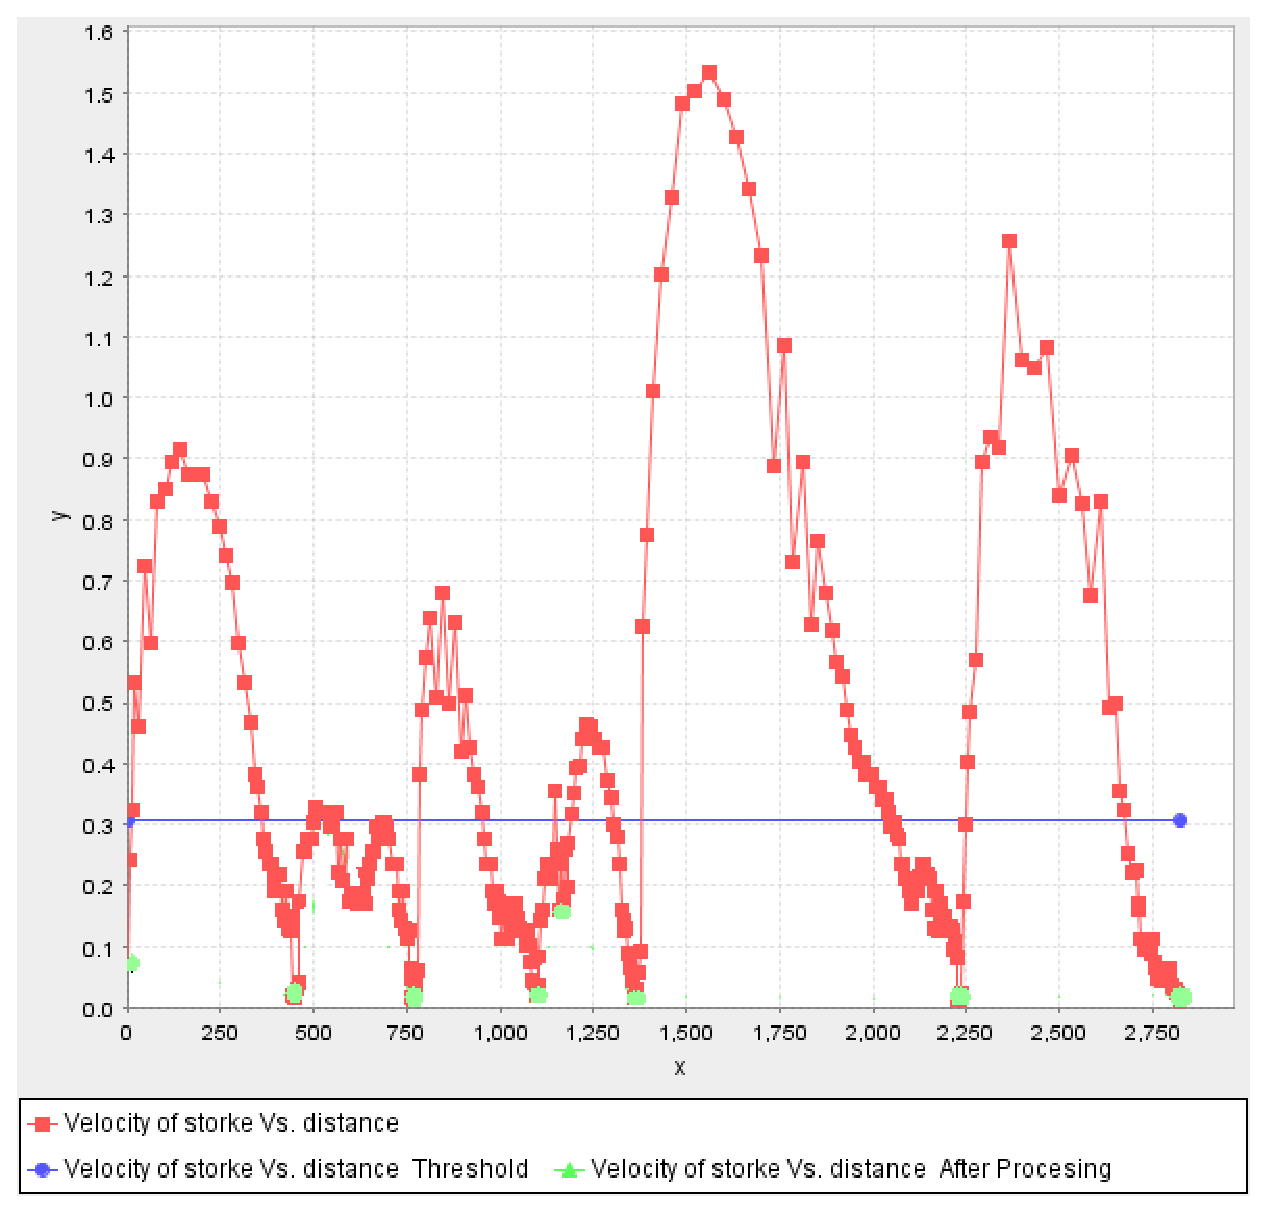
\includegraphics[scale=0.6]{images/speed2.eps}
	\caption{Speed Vs. Distance Graph}
	\label{fig:speed2Distance}
\end{figure}


\begin{figure}[]
	\centering
		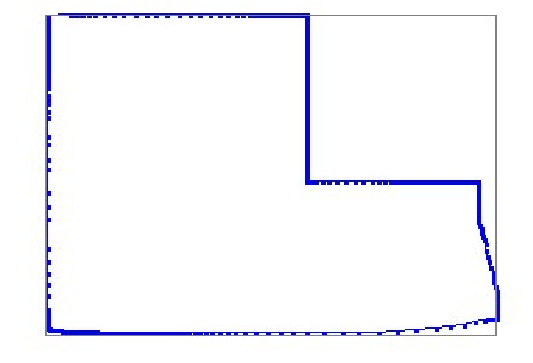
\includegraphics[scale=0.8]{images/orignalStroke.eps}
	\caption{Stroke Sample}
	\label{fig:orignalStroke}
\end{figure}




\subsection{Critical Point Detection}
\label{sec:CriticalPointDetection}
After the system computes all the speed, time difference and curvature data it proceeds to detect the points with low velocity and high curvatures. Using simple differentiations to detect local extreme points resulted in false points due to the non smooth curves. So instead the following procedure was used, firstly the mean and maximum values of the curve is computed from the actual data. 

The mean is used as threshold to divide curves values into low and high values.  This threshold is used to separate the curve into regions; each region is defined as the part between two intersection points of the threshold line and the curve.  Thus, their will be regions with value higher than the threshold   and regions with values lower than the threshold. Only regions higher than the threshold value are examined when computing the maximum of each region. The point that corresponds to those maximum values are labeled possible dominant points.  


   %After the threshold is applied the curve is divided into regions. Each region is defined by a part in the data curve between tow intersection point of the threshold line and the curve.  % to find the extreme points. Hence, the mean of the direction curve is calculated and used as threshold.   \\
   %If we tried to differentiate the curve the result will be false threshold values we divide the data into regions of data higher or lower that the threshold. This will let us only look for high data only. The maximum of each region is then computed and reported as a possible vertex point. 

   
The system repeat this process to curvature, time difference and speed curves (see fig. \ref{fig:speed2}). For each curve the points labeled as possible dominant points are saved into a single array . The points that are repeatedly labeled are given a higher score than the other points. This score is then used to sort the possible points array.  The array that contains possible points is used as input for the next stage of segmentation. 
\begin{figure}[]
%\begin{minipage}[b]{0.8\linewidth}
	\centering

	%	\subfigure[ The Speed of data] {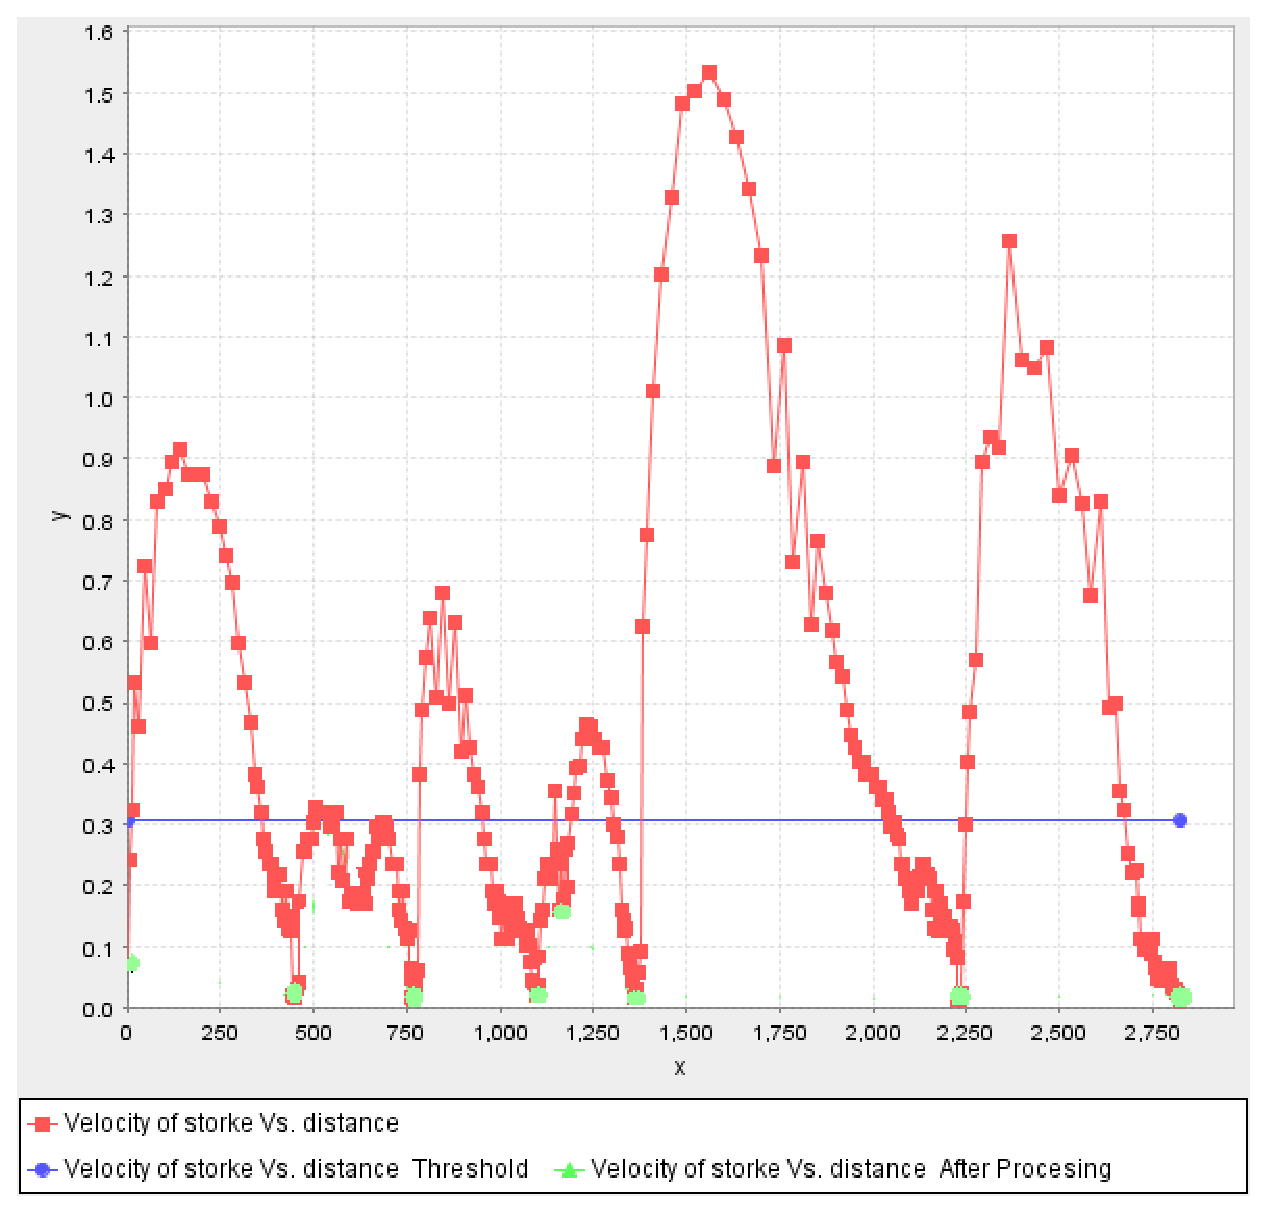
\includegraphics[scale=0.35]{images/speed2.eps}}
		
		\subfigure[ Direction ] {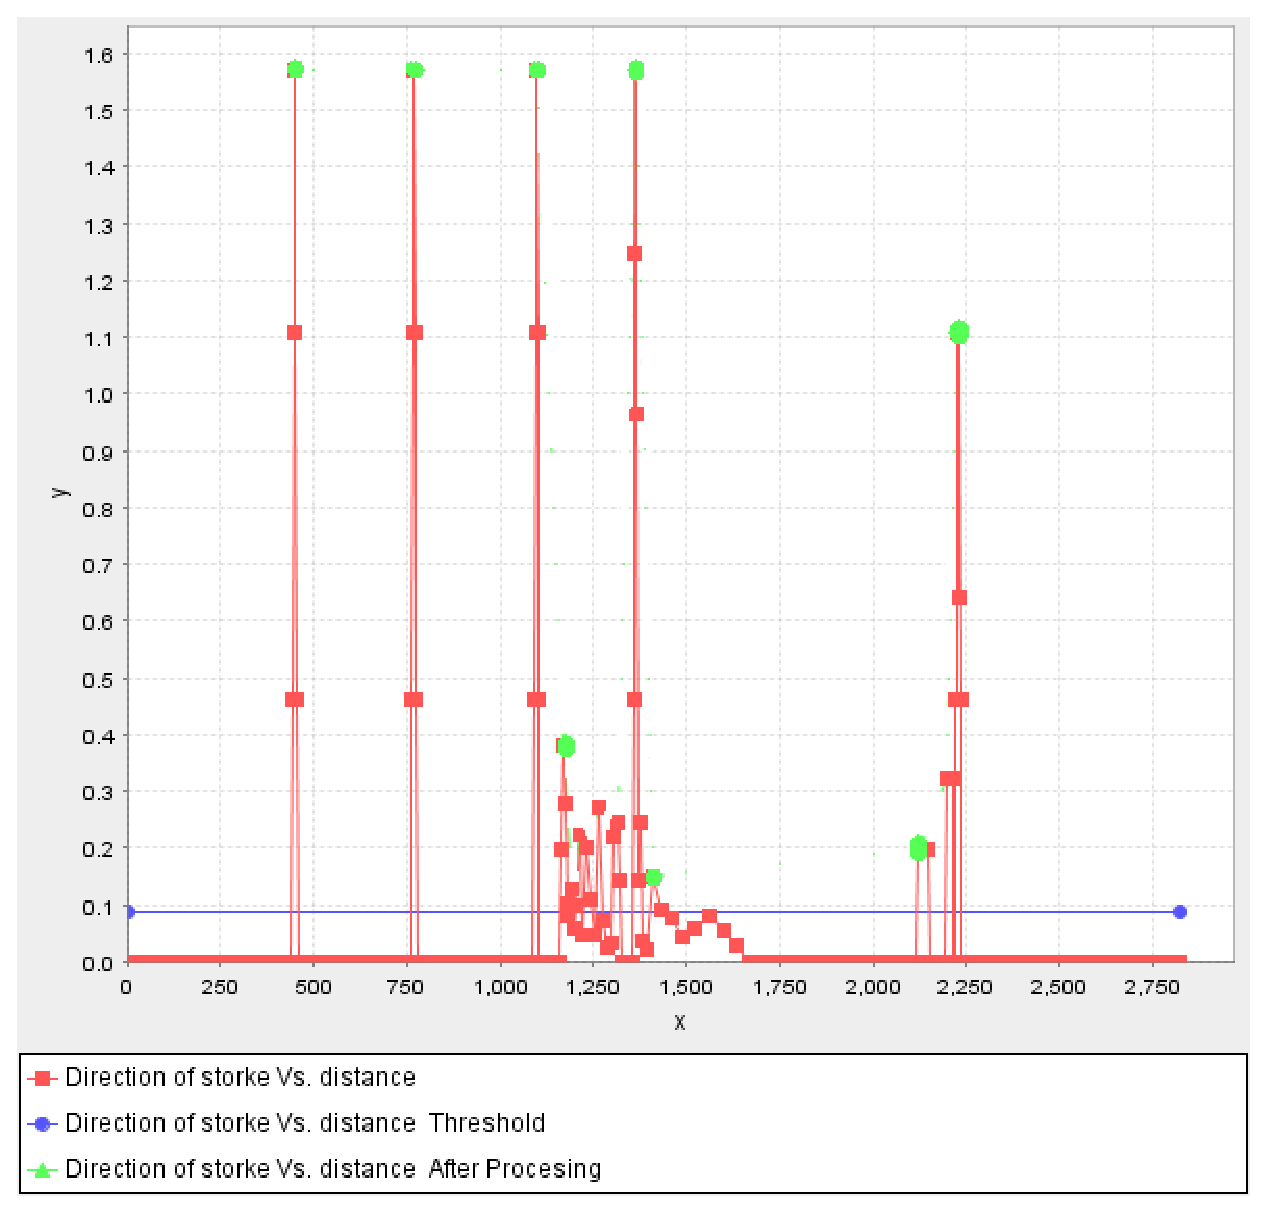
\includegraphics[scale=0.35]{images/direction2.eps}}
					%\end{minipage}
					%\begin{minipage}[b]{0.8\linewidth}
			\subfigure[Curvature] {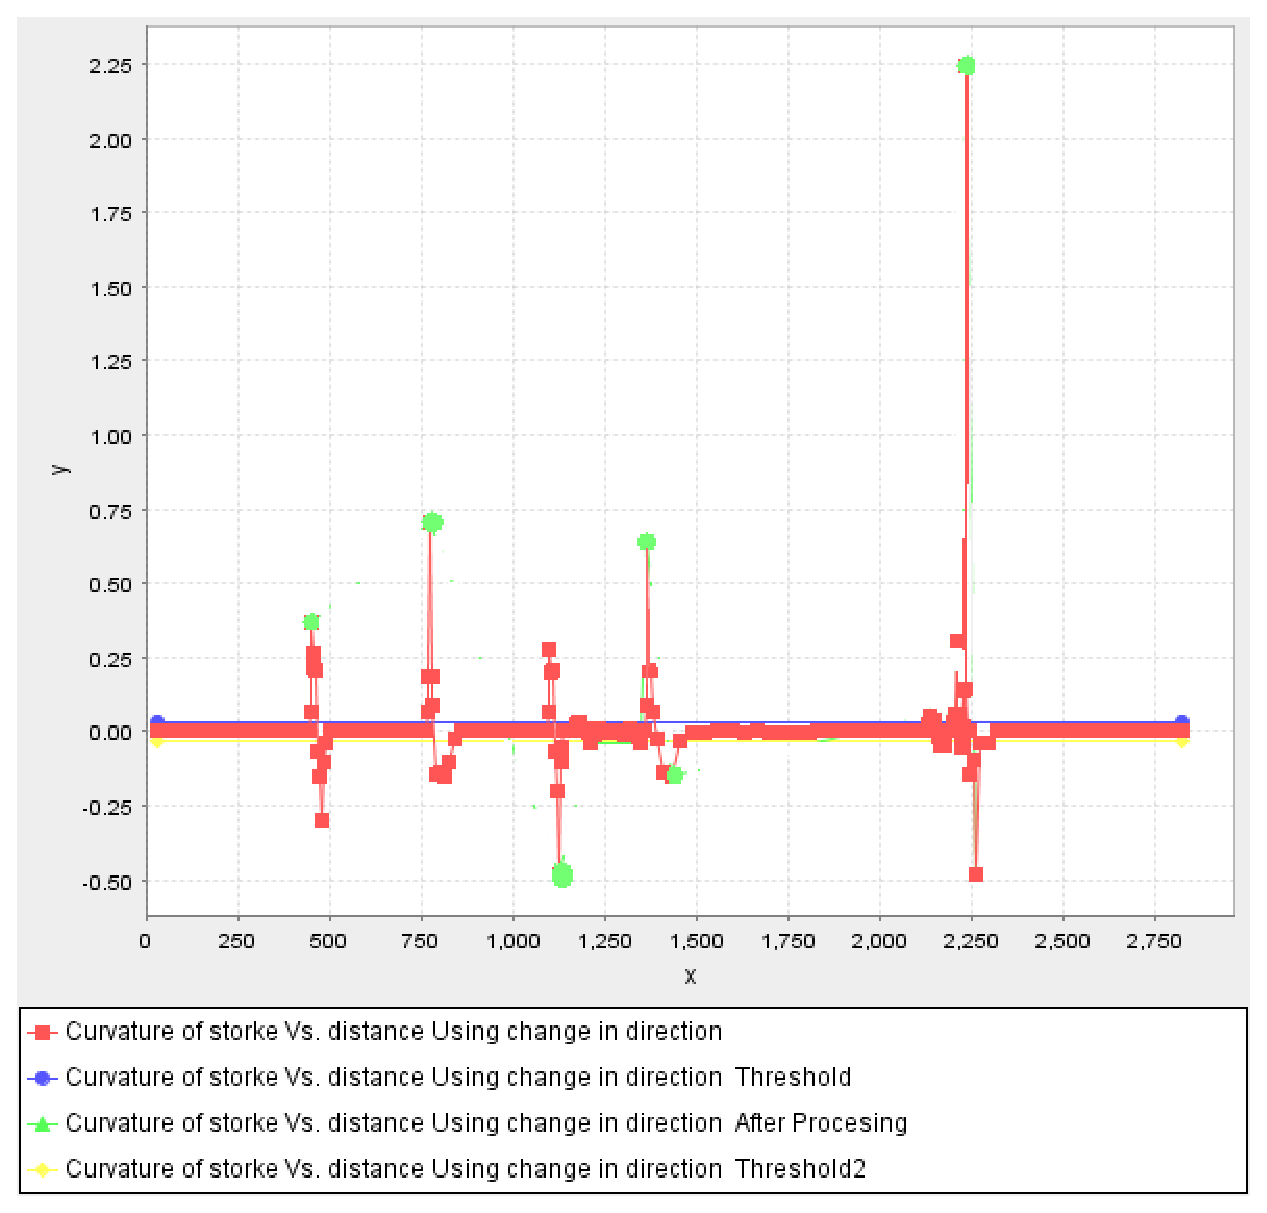
\includegraphics[scale=0.35]{images/curvature2.eps}}
			\subfigure[ Time Difference] {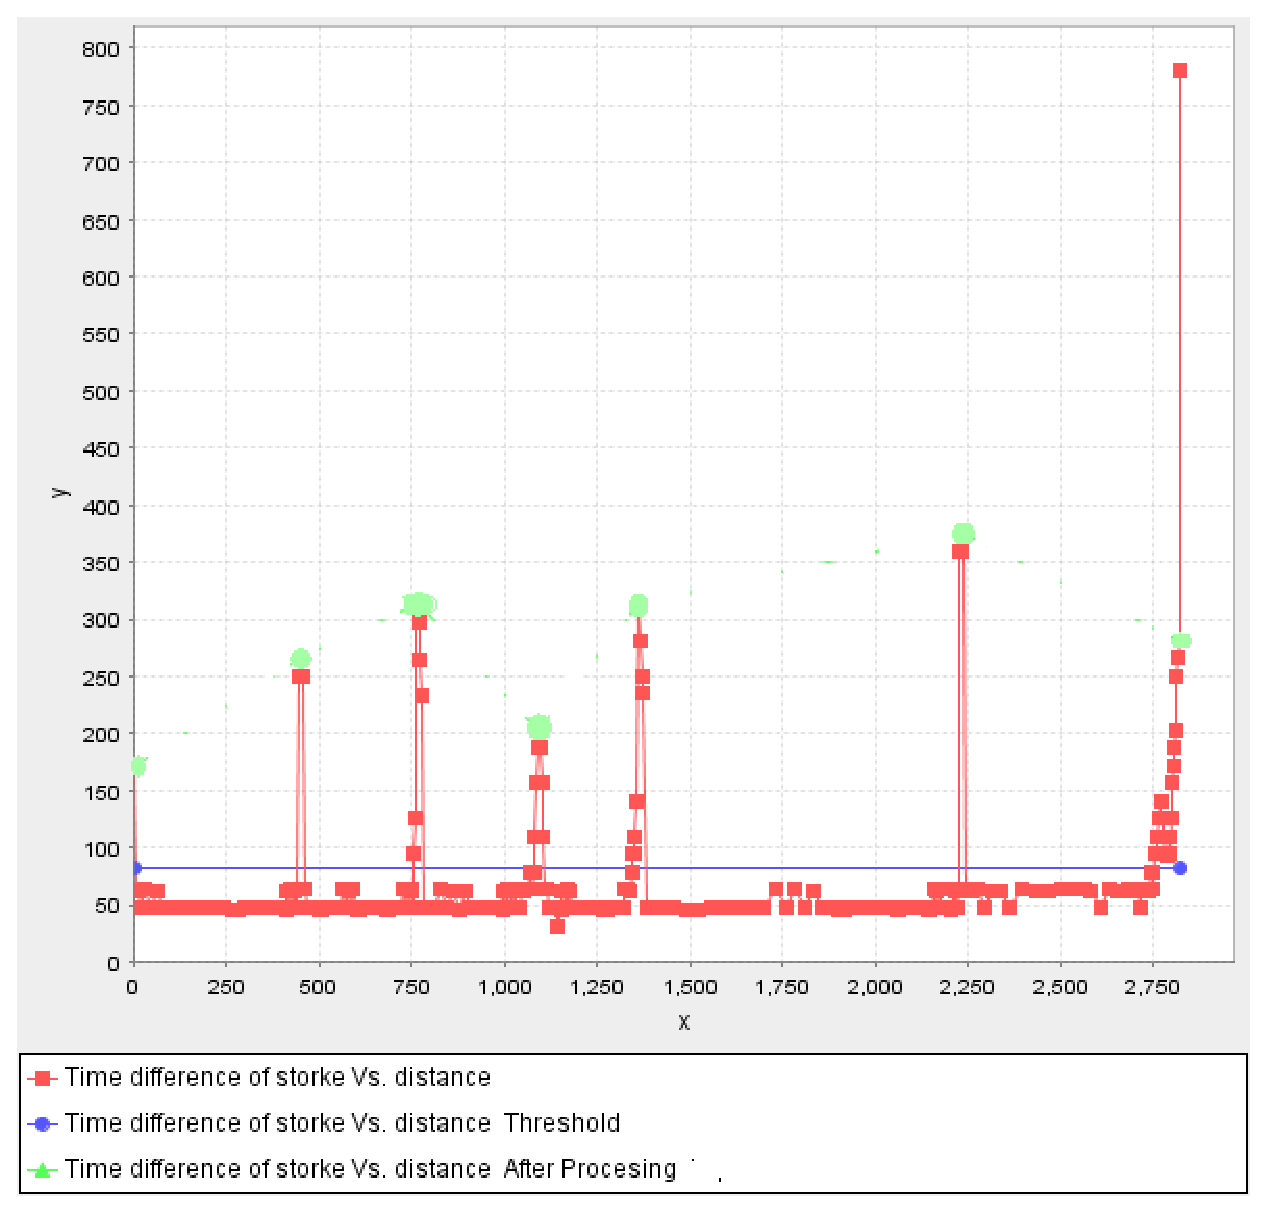
\includegraphics[scale=0.35]{images/time2.eps}}
			%\end{minipage}
	
	\caption[Data Curves]%{The data of the stroke}
	
	\label{fig:speed2}
\end{figure}

\section{Segmentation}
\label{sec:Segmentation}
The segmentation process tries to divide the stroke into a set of primitives. The segmentation algorithm first tries to detect if the stroke is an ellipse. If the stroke proved to be an ellipse then the segmentation process ends and the system proceeds to the next step. Otherwise, the stroke is passed into two particle swarm algorithms that will divide the stroke to either lines or lines and curves (see the block diagram in fig. \ref{fig:Blockdiagram} ). The algorithms takes the stroke points along with the possible dominant points computed then produce a set of dominant points which are connected with either lines or curves (see fig. \ref{fig:Blockdiagram}).  The next sections will describe the ellipse detection algorithm and both the two particle swarm algorithms used to divide the stroke.
%After computing the primary data the system now tries  \\
%Paragraphs describe the segmentation algorithm.  


\subsection{Ellipse Detection }
\label{sec:EllipseDetection}
%Describe the ellipse detection algorithms 
This process will try to fit the stroke point into an ellipse, it starts with computing the center of the stroke bounding box. The bounding box center point is used as the first estimation of the center of the ellipse. The axes of the ellipse are estimated as the $w/2$ and $h/2$ of the stroke bounding box where $w$ is width and $h$ is hight of the bonding box.  

\begin{equation}
E = \sum\limits_{i = 0}^N {\frac{{(x_i - x_0 )}}{{a^2 }}^2  + \frac{{(y_i - y_0 )}}{{b^2 }}^2  - 1} 
\label{eq:circleFit}
\end{equation}

 The least square fitting algorithm is used to minimize the fitting error of the ellipse equation (see \ref{eq:circleFit} where N is number of points in the stroke, $a,b$ are the length of ellipse axes, $x_0$ \& $y_0$ are the coordinates of the center point, $x_i$ \& $y_i$ are the coordinates of point $i$ in the stroke). A list of new values for $x_0$ , $y_0$ ,$a$ and $b$ are generated randomly from the older values with small increment and the minimum error are evalated from this list. for After only few loops the error and a confidence values  are computed.
 \begin{equation}
E = E_{ellipse}+E_{area}
\label{eq:circleError}
\end{equation}
 \begin{equation}
E_{area}  = \sqrt {\left( Area(stroke) - Area(ellipse)\right)^2 }
\label{eq:ErrorArea}
\end{equation}

   The confidence value computed by eq. ( \ref{eq:circleError}) where $E_{ellipse}$ is the error computed by eq. (\ref{eq:circleFit})  and $E_{area}$ is computed as the difference between the actual area of the stroke and the area of the estimated ellipse ( see eq.\ref{eq:ErrorArea}). The confidence value is used to label the stroke as ellipse or un segmented stroke. If the stroke as unsegmented the next process will be to pass the stroke into curve segmentation algorithm. 
   
   The next section will describe firstly the particle swarm algorithm (PSO) then it will proceed to detail the remaining of the segmentation algorithms. 
   
   %to check if the stroke can be labled as ellipse or not.\\ %is computed to check if stroke is an ellipse. \\
%We found that if the confidante is above threshold then the probability of ellipse is highest otherwise the stroke is passed to the next section to get the divisions of stroke and test its error.  


\subsection{Particle Swarm Algorithm Introduction}
\label{sec:ParticleSwarmAlgorithm}
%\section{Particle Swarm Algorithm}
%\label{PSO}
%What is particle swarm algorithm and how it was used in related researches. 
The main idea of  Particle Swarm Algorithm (PSO) is to represent each agent with a particle from the solution space. Each agent moves the particle with a direction and velocity based on the following equation [\ref{eq:Swarm}].
\begin{equation}
%\[
v_{ij}  = v_{ij}  + c_1 r_1 (lbest_{ij}  - p_{ij} ) + c_2 r_2 (gbest_{ij}  - p_{ij} )
%\]
\label{eq:Swarm}
\end{equation}
\begin{equation}
%\[
p_{ij}=p_{ij}+v_{ij},
%\]
\end{equation}
 Equation [\ref{eq:Swarm}] shows how velocity and direction of each particle is computed where $r_1$ \& $r_2$ are random variable and $c_1$ \& $c_2$ are the swarm system variables. Each iteration the global best $g_{best}$ particle and  the agent local best $l_{best}$ particle are evaluated based on the maximum fitness functions of  all particles. The solution is found after a maximum number of iteration or after an error threshold is achieved.
 \begin{equation}
   P(i)\Leftarrow 
\{
\begin{array}{c} 
1 \quad \quad if\quad r_{3}>t  \\

0 \quad \quad if\quad r_{3}<t 
\label{eq:descrite}
\end{array}\}
\end{equation}
  Equation \ref{eq:descrite} where t is a threshold and $r_{3}$  is a random variable, is used to change general swarm algorithm into binary particle which will handle particle values of either 0 or 1.  

\subsection{Swarm Segmentation}
\label{sec:SwarmSegmentation}

In this process the system generate two stroke segmentation using two PSO segmentation algorithm. The system generates segmentation from both algorithms and then chooses the segmentation with the minimum error value. The problem definition is the same in both algorithms but they differ in the fitness function and the error functions. %formation is nearly the same in both. 
\subsubsection{Problem Formulation}
\label{sec:ProblemFormulation}
The input stroke with $N$ points can be represented by set $S = \left\{ {x_1 ,x_2  \ldots x_N } \right\}$ where $x_i$ is the location of the point $i$ . The swarm algorithms consist of $M$ agents which are represented by the set 
$A  = \left\{ {P_i \left| {i = 1,2 \cdots M} \right.} \right\}$ where $P_i$ is a single solution particle from the solution space. Each particle decodes the problem with binary array with the same length $N$ as the input stroke .  
\begin{figure}
	\centering
		\includegraphics{images/CodingSwarm.eps}
	\caption{An Example Stroke and the Coding}
	\label{fig:CodingSwarm}
\end{figure}

% The particles of the swarm represent a single solution of the solution space. For this problem the, each particle %will give a different segmentation for the input stroke. Firstly, we will define the stroke with N points by the set %S where.  We define the arc %An array with the same length as the number of points of the strokes.
So the system will represent each particle $P_i$ by $P_i = \left\{ {p_{ij} \left| {j = 1,2 \cdots N} \right.} \right\}$ where $p_{ij}$ will have only two values 0 or 1 where $p_{ij}=1$ will mean that point $j$ is a dominant point(see fig. \ref{fig:CodingSwarm} ).  Thus , the particle represent which points are chosen from the set of points in the stroke to be used as dominate points for segmentation. 
The goal of the PSO algorithm is to find the solution $P_i$ that generate the minimum set of dominate points that will define the stroke with minimum segmentation error. In other words, we want to find the fewer number of points (1's) location in particle array which will gives minimum error.  


The fitness function and error calculation are different in each algorithm. The first fitness and error function is described below. 


\subsubsection{Polygon Division Algorithm}
\label{sec:PolygonDivisionAlgorithm}
For the first algorithm, the algorithm tries to segment the stroke as a polygon approximation. The final solution will be set of line segment that best define the input stroke. Given the inputs stroke let's define the set of points in the stroke as  $S = \left\{ {x_1 ,x_2  \ldots x_N } \right\}$ which is the set of consecutive points from start of stroke till the end. Then define the arc $\widehat{x_ix_j}$ as the consecutive set of points from point $x_i,x_{i+1} \cdots,x_j$. The line
$\overline{x_i x_j} $ as the straight line connecting point $x_i$ to point $x_j$. The approximation error is computed by the equation \ref{eq:ErrorSwarm1}  where M is the number of dominant points in this solution.  The error $ e ( \widehat{x_ix_j},\overline{x_i x_j})$ is computed as the sum of squared perpendicular distance from every point along the arc $\widehat{x_ix_j}$ to the line $\overline{x_i x_j}$.  \\
\begin{equation}
E=\sum\nolimits_{i = 0}^M e ( \widehat{x_ix_{i+1}},\overline{x_i x_{i+1}})
\label{eq:ErrorSwarm1}
\end{equation}
\begin{equation}
\max fitness(p_i ) = \left\{ {\begin{array}{*{20}c}
   { - E/\varepsilon N} & {ifE > \varepsilon ,}  \\
   {D/\sum\limits_{j = 1}^N {p_{ij} } } & {otherwise}  \\
\end{array}} \right.
\label{eq:fitnessSwarm1}
\end{equation}%\]

The fitness is computed using equation \ref{eq:fitnessSwarm1} where N is the number of points in the stroke, D is the number of point in the solution that was previously labeled as a possible dominant point and E is the computed error and $\varepsilon$ is the error threshold.  If the solution produced an error that exceed the error threshold the fitness function assign a -ve value for the solution to express it's in feasibility, otherwise the inverse of the number of vertex produced is used to access the solution fitness in terms of minimum number of vertices's.  This fitness function optimize two goal the first is to move the solution into the feasible solution space with accebtable error bounds and second is to fly the particle to a new position which may result in a polygon with a fewer number of vertices's. 

 %The error is chosen to in favor of larger than the threshold is given a -ve value to lower the value of solution otherwise the system will favor the lower number of vertices's.\\ %we will want to lower the number of vertices's. \\
%if we say that s
%Alg1:
%Alg2: 
\subsubsection{Curve Divisions Algorithm}
\label{sec:PolygonDivisionAlgorithm}

The second algorithm has the same problem formulation but different fitness and error functions. It was previously introduced in  \cite{CruveDivisionSwarm} where but genetic programming was used as the optimizing algorithm. The particle is represented using the arrays $P_i = \left\{ {p_{ij} \left| {j = 1,2 \cdots N} \right.} \right\}$ where $p_{ij}$ will have only two values 0 or 1 as mentioned before is section \ref{sec:PolygonDivisionAlgorithm}. Lets denote the segments $\widehat{x_ix_j}$ as the consecutive set of points from point $x_i,x_{i+1} \cdots,x_j$.  The goal of the algorithm is to fit the segments between the solution vertices's into straight lines or a circular arc. 
\paragraph{Fitting segments into straight line.}
\label{sec:FittingSegmentIntoStraightLine}
According to \cite{CruveDivisionSwarm} each segment $\widehat{x_ix_j}$ given a set of points $x_i,x_{i+1} \cdots,x_j$ can be fitted into the line: $y=kx+c$ where $k$ and $c$ are the slope and the intercept of the line respectively. Equation \ref{eq:Linek} and \ref{} are used to fit the segment $\widehat{x_ix_j}$ into the straight line where N is the number of points in the segment and $(x_i, y_i)$ are the coordinate of the point $i$. 

\begin{equation}
\label{eq:Linek}
k = \frac{{N\sum\limits_{i = 1}^N {x_i y_i }  - \sum\limits_{i = 1}^N {x_i } \sum\limits_{i = 1}^N {y_i } }}{{N\sum\limits_{i = 1}^N {x_i^2 }  - \left( {\sum\limits_{i = 1}^N {x_i } } \right)^2 }}
\end{equation}
\begin{equation}
\label{eq:LineC}
c = \frac{{\sum\limits_{i = 1}^N {x_i^2 } \sum\limits_{i = 1}^N {y_i }  - \sum\limits_{i = 1}^N {x_i } \sum\limits_{i = 1}^N {x_i y_i } }}{{N\sum\limits_{i = 1}^N {x_i^2 }  - \left( {\sum\limits_{i = 1}^N {x_i } } \right)^2 }}
\end{equation}
\begin{equation}
\label{eq:ds}
 d_s  = \frac{{\sum\limits_{i = 1}^N {\left| {(kx_i  + c) - y_i } \right|} }}{{N\sqrt {k^2  + 1} }}
\end{equation}

The distance($d_s$) (see equation \ref{eq:ds}) is the average distance from segment points $(x_i, y_i)$ to the  line estimated. This distance ($d_s$) is used to estimate the error of the line approximation which we will dnote as ($E_s$). 


\paragraph{Fitting segments into circular arc.}
\label{sec:FittingSegmentcirculararc}
The segment points can also be fitted into the circular arc $(x - a)^2  + (y - b)^2  = R^2, $ where ($a,b$) are the coordinate of the center of the circle and $R$ is the radius of the circle. They can be estimated using the following set of equations: 
 
\begin{equation}
a = \frac{{b_{1}a_{22} - b_{2}a_{12}}}{\Delta},
\end{equation}
\begin{equation}
	b = \frac{{b_{2}a_{11} - b_{1}a_{21}}}{\Delta},
\end{equation}
\begin{equation}
R = \sqrt {\frac{1}{N}(\sum\limits_{i = 1}^N {x_i^2 }  - 2\sum\limits_{i = 1}^N {x_i a}  + Na^2  + \sum\limits_{i = 1}^N {y_i^2  - 2} \sum\limits_{i = 1}^N {y_i b + Nb^2 } )} ,
\end{equation}

Where 
\begin{equation}
a_{11}  = 2\left[ {\left( {\sum\limits_{i = 1}^N {x_i } } \right) - N\sum\limits_{i = 1}^N {x_i^2 } } \right]
\end{equation}
\begin{equation}
a_{12}  = a_{21}  = 2\left( {\sum\limits_{i = 1}^N {x_i \sum\limits_{i = 1}^N {y_i } }  - N\sum\limits_{i = 1}^N {x_i y_i^2 } } \right),
\end{equation}
\begin{equation}
 a_{22}  = 2\left[ {\left( {\sum\limits_{i = 0}^N {y_i } } \right)^2  - N\sum\limits_{i = 0}^N {y_i^2 } } \right]
\end{equation}
\begin{equation}
b_1  = \sum\limits_{i = 0}^N {x_i^2 } \sum\limits_{i = 0}^N {x_i }  - N\sum\limits_{i = 0}^N {x_i^3 }  + \sum\limits_{i = 0}^N {x_i } \sum\limits_{i = 0}^N {y_i^2 }  - N\sum\limits_{i = 0}^N {x_i y_i^2 } , 
\end{equation}
\begin{equation}
b_2  = \sum\limits_{i = 0}^N {x_i^2 } \sum\limits_{i = 0}^N {y_i }  - N\sum\limits_{i = 0}^N {y_i^3 }  + \sum\limits_{i = 0}^N {y_i } \sum\limits_{i = 0}^N {y_i^2 }  - N\sum\limits_{i = 0}^N {x_i^2 y_i } ,
\end{equation}

\begin{equation}
\Delta  = a_{11}b_{22}-a_{12}a_{21}.
\end{equation}
 The error of the circle estimated is measured using the distance ($d_c$) which is calculated using the following equation:
 \begin{equation}
 \label{eq:circleE}
d_c  = \frac{{\sum\limits_{i = 0}^N {\left| {\sqrt {(x_i  - a)^2  + (y_i  - b)^2 }  - R} \right|} }}{N}
\end{equation}
Thus, eq.(\ref{eq:circleE}) ($d_c$) define the average distance ($d_c$) from the segment points ($x_i,y_i$) to the estimated fitted circle ($a,b$) and $R$.

\paragraph{Determinig The Segment Type.} 
\label{sec:DeterminigSegmentType}
If the average distance ($d_s$) equalls zero that means that the segments point is exactly the straight line approximated. If the distance ($d_c$) equals zero means that the segments point lies exactly on the circular arc estimated. But the user rarely draws an exact line or circle, so the distances are used as the error estimations. The distance will determine the type of the current segment, in other words if ($d_s$) is smaller than ($d_c$) then the segment is labeled as a line segment otherwise it is labeled as a circular arc. \\


After each segment type is determined the the particle segmentation error is computed by the equation equation \ref{eq:errorSwarm2} where M is the number of segments in the solution, $D_i$ is the  approximation error of each segment as $min(d_c,d_s)$ as computed in eq.(\ref{eq:circleE})  and eq. (\ref{eq:ds})  \cite{CruveDivisionSwarm}. The fitness is computed by the equation \ref{eq:fitnessSwarm2} where E is the error and M is number of segments and k is a parameter tweaked to get minimum number of segments.




 %and line estimation are computed for each segment, the approximation with the lower error value will be the chosen approximation of this segment. The sum of the approximation error of all segments is the total error of the particle.  The error is computed by   \\
 
 
\begin{equation}
E=\sum\nolimits_{i = 0}^M e(D_i) 
\label{eq:errorSwarm2}
\end{equation}
\begin{equation}
\max fitness(P_i ) = \frac{1}{{E \times M^k }}
\label{eq:fitnessSwarm2}
\end{equation}



%Describe how we used particle swarm in curve polygon approximation using first algorithm.  
%Describe how we used PSO in to divide stroke into segments and curves. 
%[These two algorithm was modified from the algorithm in paper \cite{PolygonApproximationPSO,CruveDivisionSwarm}].
\cite{PolygonApproximationPSO} used a merge and divide algorithm after each loop of the swarm system to refine the solution but we used another enhancement method. After each loop in the swarm algorithm, each particle loops on the set of selected dominant points to enhance the solution. Each dominant point is checked to find if it was labeled before as a possible dominant (computed as in section \ref{Prepross}), if not the point is moved to the nearest labeled point.    
%check the new solution and check the new vertices's if a vertex points is a possible dominant point it is left as a vertex. Otherwise, the system will search in the local neighborhood for the nearest possible dominant point to move these vertices's to. After each change the error is computed and if new error is less that the old then the new set is approved. \\
\section{BenchMarck algorithm}
\label{sec:BenchMarckAlgorithm}
In this research, a bench mark algorith is used to compare to results obtained by the PSO algorithms. The algorithm was first implemented by  \citeauthor{earlyprocess} in \cite{earlyprocess}. The \citeauthor{earlyprocess} algorithms is divided into the following steps. 
\begin{enumerate}
	\item compute the curvatures and the speed of the stroke points. 
	\item Threshold the curvature and speed curves using a percentage of the maximum value in the curve. 
	\item Mark the values higher than the threshold in an new arrays $L_c$ for list of corner points generated from the curvature curve. The list $L_s$ contains the points generated from the speed curve.
	\item Compute a confidence on each list based on the type of curve. Then sort the lists $L_s$and $L_c$ by the confidence value. 
	\item Find the intersection points in both list and generate the a Sample solution $h_{curr}$. 
	\item Use $h_{curr}$ as initial solution. Loop doing the following:
	
		\begin{enumerate}
			\item Generate a new solution $h_{s}$ using $h_{curr}$ and  the first point from the $L_s$ list .
			\item Generate a new solution $h_{c}$ using $h_{curr}$ and  the new point from the $L_c$ list.
			\item Test the solutions $h_{s},h_c$ to find the minium solution.
			\item  If $h_s$ then add the solution a list of hybrid solutions $Solutions_{set}$ and remove the first point from the list $L_s$ then set $h_s$ as $h_{curr}$. 
			\item If $h_c$ then add the solution a list of hybrid solutions $Solutions_{set}$ and remove the first point from the list $L_c$ then set $h_c$ as $h_{curr}$. 
		\end{enumerate}
		\item Choose the final solution from the list of solutions $Solutions_{set}$ as a trade off between  minimum error and number of corners.  
		\item Check each segment in the solution if the solution is can be estimated as a line segment if not it is fitted using a higher level Bezire curve. 
\end{enumerate}
More details about the algorithm is in \cite{earlyprocess}.


\section{Stroke Clustring Algoirthm }
\label{sec:ClustringAlgoirthm}

When the user finish drawing a stroke the segmentation algorithm generate a list of segments that represent this stroke. The clustering algorithms group the segments generated from the segmentation algorithm. These segments are grouped into a symbol and tested if they can be classified into one of the known symbols. If no identification is achieved the segments are added into a list of unclassified segments. When a user draws another stroke the segmented stroke is added to the list and the process is repeated until all the segments are classified to a known symbol.\\

After the user draw all strokes of the symbol he has to wait 10 seconds or press finish button beside the drawing area. The set of unrecognized strokes is grouped together along with their segmentation as input to the feature extraction process. 

\section{ Feature Extraction}%%Feature Set
\label{sec:FeatureExtraction}

The system uses a composite set of features include Rubine feature set \cite{gestureexample12}, Zernike moments \cite{HeloiseBeautification}, ink density \cite{GeometryAndDomain102} and some structural information like number of perpendiculars lines , number of parallel lines and types of primitives in each symbol. The table \ref{tab:FeatureTable} gives details on all the features used in the system.
 %trained with the 13 categories in the system. The same training set was used by \cite{HeloiseBeautification} in their symbol recognition system. \\ %  The table describe the features used in the system. 
%\begin{table}
%\begin{minipage}[t][1\totalheight]{0.3\columnwidth}
%
%\begin{tabular}{|l|l|l|l|}
%\hline 
%Type & index & Features & Notes\tabularnewline
%\hline 
%\hline Structural & F1. & No. of parallel lines & \tabularnewline
%\hline & F2. &  No. of perpendicular lines & \tabularnewline
%\hline & F3. &  No. of intersections between any two segments. & \tabularnewline
%
%\hline Statistical& F4.and F5. & Mean and standard deviation of the Curvature data   & \tabularnewline
%\hline & Mean of the speed data & \tabularnewline
%\hline 
%Rubine & Set of features \\for gesture recognition & Introduced by Rubine in \cite{} \tabularnewline
%\hline Zernike &  A Zernike\\ moments  &  Used by \cite{zernike61} \tabularnewline
%\hline Composite & width to\\ height ratio  & \tabularnewline
%\hline  & ink density  & Used by \cite{} \tabularnewline
%\hline
%\end{tabular}		
%\end{minipage}
%	\caption{Feature Table}
%	\label{tab:FeatureTable}
%\end{table}





%\begin{table}
%\begin{tabular*}{0.5\textwidth}{|l|l|l|l|}
%\begin{tabular}{|l|l|p{6cm}|p{5cm}|}
%\hline
%Type & Index & Features & Notes \\ 
%\hline
%Structural & \multicolumn{1}{c|}{} &  &  \\ 
%\hline
% & F1. & No. of parallel lines &  \\ 
%\cline{2-4}
% & F2. & No. of perpendicular lines &  \\ 
%\cline{2-4}
% & F3. & No. of intersection between of any two segmetns  &  \\ 
%\cline{2-4}
% & F4.  & No of primitives  &  \\ 
%\cline{2-4}
% & F5.  & No. of line segments &  \\ 
%\cline{2-4}
% & F6 & No. of ellipse, circular arcs.  &  \\ 
%\hline
%Statistical &  &  &  \\ 
%\hline
% & F7.  &  &  \\ 
%\cline{2-4}
% & F8. &  &  \\ 
%\hline
%Rubine Features &  & From features F9. till F13  & Introduced by in \cite{gestureexample12} \\ 
%\hline
% & F9. & Cosine of starting angle &  \\ 
%\cline{2-4}
% & F10. & Sine of starting angle &  \\ 
%\cline{2-4}
% & F11.  & Length of diagonal of bounding box 
% & (gives an idea of the size of the bounding box) \\ 
%\cline{2-4}
% & F12. & Angle of diagonal
%  & gives an idea of the shape of the bounding box (long, tall, square)
%  \\ 
%\cline{2-4}
% & F13. & Distance from start to end
% &  \\ 
%\cline{2-4}
% & F14. & Cosine of ending angle
% &  \\ 
%\cline{2-4}
% & F15. & Sine of ending angle  &  \\ 
%\cline{2-4}
% & F16. & Total stroke length
% &  \\ 
%\cline{2-4}
% & F & Change in Rotation( Arctan )& gives the directional angle \\ 
%\cline{2-4}
% & F & Absolute rotation 
% &  \\ 
%\cline{2-4}
% & F & Rotation squared 
% &  \\ 
%\cline{2-4}
% & F & The maximum speed reached (squared)
% &  \\ 
%\cline{2-4}
% & F & Total time of stroke
%  &  \\ 
%\hline
%Zernike moments &  &  &  \\ 
%\hline
% & F & Zernike moments to the n order &  used by \cite{zernike61} \\ 
%Composite  &  &  &  \\ 
%\hline
% &  &  &  \\ 
%\cline{2-4}
% &  &  &  \\ 
%\cline{2-4}
% &  &  &  \\ 
%\hline
%\end{tabular}


%\newpage

%\begin{table}
\begin{longtable}{|l|l|p{6cm}|p{5cm}|}
	%\caption{Feature Table}
	%\label{tab:FeatureTable}
\hline 
Type  & Index  & Features  & Notes \tabularnewline
\endhead
\hline 
Type  & Index  & Features  & Notes \tabularnewline
\endfirsthead
\hline 
Structural  & \multicolumn{1}{c||}{} &  & \tabularnewline
\hline 
 & F1.  & No. of parallel lines  & \tabularnewline
\hline 
 & F2.  & No. of perpendicular lines  & \tabularnewline
\hline 
 & F3.  & No. of intersection between of any two segmetns  & \tabularnewline
\hline 
 & F4.  & No of primitives  & \tabularnewline
\hline 
 & F5.  & No. of line segments  & \tabularnewline
\hline 
 & F6  & No. of ellipse, circular arcs.  & \tabularnewline
\hline 
Statistical  &  &  & \tabularnewline
\hline 
 & F7.  &  & \tabularnewline
\hline 
 & F8.  &  & \tabularnewline
\hline 
Rubine Features  &  & From features F9. till F13  & Introduced by in \cite{gestureexample12} \tabularnewline
\hline 
 & F9.  & Cosine of starting angle  & \tabularnewline
\hline 
 & F10.  & Sine of starting angle  & \tabularnewline
\hline 
 & F11.  & Length of diagonal of bounding box  & (gives an idea of the size of the bounding box) \tabularnewline
\hline 
 & F12.  & Angle of diagonal  & gives an idea of the shape of the bounding box (long, tall, square) \tabularnewline
\hline 
 & F13.  & Distance from start to end  & \tabularnewline
\hline 
 & F14.  & Cosine of ending angle  & \tabularnewline
\hline 
 & F15.  & Sine of ending angle  & \tabularnewline
\hline 
 & F16.  & Total stroke length  & \tabularnewline
\hline 
 & F  & Change in Rotation( Arctan ) & gives the directional angle \tabularnewline
\hline 
 & F  & Absolute rotation  & \tabularnewline
\hline 
 & F  & Rotation squared  & \tabularnewline
\hline 
 & F  & The maximum speed reached (squared)  & \tabularnewline
\hline 
 & F  & Total time of stroke  & \tabularnewline
%\newpage
\hline 
Zernike moments  &  &  & \tabularnewline
\hline 
 & F  & Zernike moments to the n order  & used by \cite{zernike61} \tabularnewline
Composite  &  &  & \tabularnewline
\hline 
 &  &  & \tabularnewline
\hline 
 &  &  & \tabularnewline
\hline 
 &  &  & \tabularnewline
\hline
\end{longtable}
%\end{table}
  % Rubine el al.\cite{gestureexample12}  used a set of statistical features,  There are a lot of features used in the sketch recognition literature
%How to handle multi-stroked symbols. 
%The clustering algorithm.  
%The classifier used in recognition
%Describe the features used in recognition [ref to \cite{zernike61}]

\section{Classification}%%Feature Set
\label{sec:Classification}
 After computing the features the symbol is introduced to the classifier. The system used a support vector machine (SVM) classifier with Gaussian kernel (RBF kernel) \cite{libsvm}. The system used (object versus all) OVA classifiers structures. A validation algorithm used to choose the Kernel variables parameters  $c,\gamma$ to be used in the SVM classifiers. The Rubine algorithm (Linear Gaussian classifier ) was implemented for comparing the system. The results section \ref{} demonstrates the results of both classifiers. \\%Some features like number of parallel, perpendicular and intersecting lines are computed from the segmentation other like density, centroid and Zernike moments are computed from the raw stroke points. 

%%%%%%%%%%%%%%%%%%%55555555
%Symbol Recognition 16
%4.1 Preprocessing and segmentation . . . . . . . . . . . . . . . . . . . . . . . . . . . 16
%4.2 Feature-Based Statistical Symbol Recognition . . . . . . . . . . . . . . . . . . . . 18
%4.2.1 Feature Set . . . . . . . . . . . . . . . . . . . . . . . . . . . . . . . . . . 19
%4.2.2 Training . . . . . . . . . . . . . . . . . . . . . . . . . . . . . . . . . . . . 21
%4.2.3 Recognition . . . . . . . . . . . . . . . . . . . . . . . . . . . . . . . . . . 23
%4.2.4 User Study . . . . . . . . . . . . . . . . . . . . . . . . . . . . . . . . . . 24
%4.3 Graph-Based Symbol Recognition . . . . . . . . . . . . . . . . . . . . . . . . . . 28
%4.3.1 Previous Work . . . . . . . . . . . . . . . . . . . . . . . . . . . . . . . . 28
%4.3.2 Statistical Graph Definitions and Error-driven Stochastic Graph Matching . 29
%4.4 Image Based Symbol Recognition . . . . . . . . . . . . . . . . . . . . . . . . . . 30
%4.4.1 User Study . . . . . . . . . . . . . .
%3.3 System Components 43
%4 Segmenting a Freehand Sketch
%4.1 Interface 51
%4.2 Spline representation 52
%4.3 Points of potential feature separation 59
%4.4 Corner detection 59
%4.5 Intersection detection 61
%4.6 Clustering of interesting points 65
%4.7 Feature Extraction